\documentclass[10pt,a4paper]{article}
\usepackage[italian]{babel}
\usepackage[utf8]{inputenc}
\usepackage{amsmath}
\usepackage{amsfonts}
\usepackage{amssymb}
\usepackage{a4wide}
\usepackage{graphicx}
\usepackage{todonotes}
\usepackage[toc]{glossaries}

\makeglossaries

\newglossaryentry{Ingegneria del Software}
{
	name={Ingegneria del Software},
	description={Approccio sistematico, disciplinato e quantificabile allo sviluppo, il mantenimento e il ritiro del software}
}

\newglossaryentry{best practice}
{
	name={best practice},
	description={Metodo di lavoro che l'esperienza e lo studio hanno provato avere i migliori risultati in circostanze specifiche e ben note}
}

\newglossaryentry{efficienza}
{
	name=efficienza,
	description={Valore indicativo inversamente proporzionale alla quantità di risorse consumate nell'esecuzione di un processo di produzione}
}

\newglossaryentry{efficacia}
{
	name=efficacia,
	description={Valore indicativo di quanto un prodotto o un processo soddisfano i requisiti di conformità e qualità}
}

\newglossaryentry{ciclo di vita}
{
	name={ciclo di vita},
	description={Insieme di tutti gli stati assunti dal prodotto dal concepimento al ritiro, e dei processi che lo portano da uno stato all'altro}
}

\newglossaryentry{stakeholder}
{
	name=stakeholder,
	description={Soggetto (o un gruppo di soggetti) influente nei confronti di un'iniziativa economica, sia essa un'azienda o un singolo progetto}
}

\newglossaryentry{processo}
{
	name={processo},
	description={Struttura metodologica, normativa e strategica che caratterizza, suddivide e ordina le attività di progetto}
}

\newglossaryentry{milestone}
{
	name={milestone},
	description={Stato del progetto in cui e' possibile accertare un progresso significativo}
}

\newglossaryentry{metrica}
{
	name=metrica,
	description={Sistema di misurazione}
}

\newcommand{\strong}[1]{\textbf{#1}}
\newcommand{\frgnword}[1]{\textit{#1}}

\title{Ingegneria del Software}
\author{Filippo Sestini}

\begin{document}
\maketitle
\tableofcontents

\section{Introduzione}
\subsection{Ingegneria del Software}
L'Ingegneria è l'applicazione di principi matematici e fisici per fini pratici. Tali fini sono spesso di interesse sociale e civile, non solo legati a prodotti di consumo. L'\strong{\gls{Ingegneria del Software}} è l'approccio sistematico, disciplinato e quantificabile allo sviluppo, il mantenimento e il ritiro del software. È sistematico e disciplinato in quanto fatto secondo un piano prefissato o un insieme di regole in modo metodico e standardizzato. È quantificabile perchè si vuole che il costo di un processo, in termini di tempo e denaro in particolare, sia noto a priori.

L'ingegnere del software segue una \frgnword{\gls{best practice}}, un metodo di lavoro che l'esperienza e lo studio hanno provato avere i migliori risultati in circostanze specifiche e ben note.

L'Ingegneria del Software è strettamente correlata alle seguenti discipline:
\begin{itemize}
	\item Informatica: l'Ingegneria del Software non è una branca dell'Informatica, ma una disciplina ingegneristica che si appoggia in parte su essa;
	\item Matematica: analisi numerica, matematica discreta, ricerca operativa, statistica, ecc.;
	\item Economia e management;
	\item Psicologia e sociologia;
\end{itemize}

L'ingegnere del software deve assicurare la qualità del prodotto richiesta dai requisiti, massimizzando l'\strong{\gls{efficacia}} dei processi, contenendo i costi e i tempi di produzione e minimizzando l'uso di risorse, massimizzandone quindi l'\strong{\gls{efficienza}}. I valori di efficienza ed efficacia sono inversamente proporzionali: la migliore soluzione al problema (tipicamente ve n'è più di una) tenderà ad avere valori ottimi per entrambi.

Vi sono più tipi di prodotti software: prodotti generici, \frgnword{stand-alone}, prodotti da aziende di sviluppo software e messi apertamente sul mercato, e prodotti specifici, commissionati da un particolare cliente.

Ogni prodotto software ha un \strong{\gls{ciclo di vita}}, che rappresenta tutti gli stati assunti dal prodotto dal concepimento al ritiro. Durante il loro ciclo di vita, molti sistemi software sono soggetti a varie forme di \strong{manutenzione}, che può essere di tre tipi:

\begin{itemize}
	\item Correttiva: corregge eventuali difetti riscontrati;
	\item Adattiva: modifica il software per riflettere eventuali richieste del cliente o variazioni nel mercato;
	\item Evolutiva: aggiunge nuove funzionalità al sistema;
\end{itemize}

La mantenibilità è una qualità essenziale del software.

\subsection{Il \frgnword{software engineer}}
L'ingegnere del software implementa parti di un sistema complesso conscio del fatto che altre persone potranno in futuro usarlo, completarlo o modificarlo. È necessario per lui comprendere il contesto in cui è posto il sistema che contribuisce a sviluppare.

L'ingegnere del software è guidato da alcuni principi etici:
\begin{itemize}
	\item Considerare la qualità come obbiettivo primario;
	\item Aiutare il cliente a comprendere ciò di cui ha veramente bisogno;
	\item Scegliere i processi più adatti al progetto;
	\item Ridurre la distanza intellettuale tra il software e il problema da risolvere;
	\item Essere proattivo nella ricerca degli errori;
	\item Motivare, formare e far crescere professionalmente le persone;
\end{itemize}

% L'evoluzione tecnica e tecnologica può essere d'aiuto nell'affrontare problematiche accidentali, ma non può evitare di scontrarsi con problemi essenziali (vedi \emph{No Silver Bullet -- Essence and Accidents of Software Engineering, Brooks})

\subsection{Le persone}
Con il termine \strong{\frgnword{\gls{stakeholder}}} (o portatore di interesse) si individua un soggetto (o un gruppo di soggetti) influente nei confronti di un'iniziativa economica. Un progetto software coinvolge diverse tipologie di \frgnword{stakeholder}, tra cui:

\begin{itemize}
	\item \frgnword{Business management}: chi fissa gli obbiettici in termini di costi, profitti e priorità strategiche;
	\item \frgnword{Project management}: chi gestisce le risorse del progetto e comunica con l'azienda e il committente;
	\item Team di sviluppo: chi implementa il prodotto. Qui lavora il \frgnword{software engineer};
	\item Clienti: chi compra il prodotto;
	\item \frgnword{End users}: chi utilizza il prodotto;
\end{itemize}

\subsection{Il progetto}
Un progetto software è un insieme delle attività (insieme di compiti) di produzione del software. È permeato dal principio `\frgnword{by construction}' più che da quello `\frgnword{by correction}': il prodotto è creato sapendo fin dall'inizio che funzionerà.


Un progetto è una serie di passi precisi:
\begin{itemize}
	\item Pianificazione: pianificare ciò che deve essere fatto, organizzare e controllare il tempo a disposizione, le risorse e i risultati;
	\item Analisi dei requisiti: comprendere il problema e definire cosa bisogna fare per risolverlo, e quali risorse sono necessarie;
	\item Progettazione: definire in forma concreta la soluzione, e come raggiungerla;
	\item Realizzazione: arrivare alla soluzione con il massimo valore di efficienza ed efficacia, aderendo pienamente ai requisiti;
	\item Verifica e validazione: garantire che ciò che si è fatto soddisfa i requisiti e non contiene difetti;
	\item Manutenzione: assicurare la piena usabilità del software fino al suo ritiro;
\end{itemize}

\subsection{Il processo}
Il \strong{\gls{processo}} è la struttura metodologica, normativa e strategica che caratterizza le attività di progetto. Esso suddivide le attività per obbiettivi, definendo come esse interagiscano tra loro e in che ordine debbano essere completate.

%\section{Processi software}
%\subsection{Processi, modelli, progetti}
%\subsection{Principio di miglioramento continuo}

\section{Ciclo di vita del software}
Il ciclo di vita di un prodotto software può essere visto come una macchina a stati, dove ogni stato rappresenta un preciso grado di maturazione del prodotto, e dove ogni transizione tra stati richiede l'esecuzione di attività, raggruppate in processi. Ogni prodotto software, lungo il suo ciclo di vita, attraversa gli stati di concepimento, sviluppo, utilizzo e ritiro.

Stati e transizioni hanno precise pre- e postcondizioni, determinate da vincoli, regole e strategie dedicate. La durata temporale entro uno stato di ciclo di vita o in una transizione tra essi viene detta \strong{fase}. Le fasi mostrano l'avanzamento del progetto in funzione del tempo trascorso.

\subsection{Modelli di ciclo di vita}
I modelli di ciclo di vita del software enfatizzano i processi chiave da attuare e le relazioni e interdipendenze logiche e temporali tra di essi. Il modello di ciclo di vita adottato pone vincoli su pianificazione e gestione del progetto. Esso è indipendente da metodi e strumenti di sviluppo, e precede la loro selezione. L'ingegnere del software deve essere a conoscenza del ciclo di vita da adottare in modo da stimare costi, tempi, vincoli e benefici fin dall'inizio.

\subsubsection{Modello sequenziale (\frgnword{Waterfall model})}
Il modello a cascata (o \frgnword{Waterfall model}) è un modello sequenziale nel quale il processo di realizzazione del software è strutturato in una sequenza strettamente lineare di passi, in cui il ritorno a fasi precedenti non è permesso. Al completamento di ogni passo è prodotta della documentazione, che permette al cliente di analizzare lo stato di avanzamento e approvarlo (\frgnword{document-driven model}). La fase successiva non può iniziare fintanto che quella precedente non è conclusa e approvata.

Questo modello ha origine nell'industria manufatturiera, dove i cambiamenti in corso d'opera hanno costi proibitivi e sono difficilmente attuabili.

Ogni passo del modello a cascata è definito in termini di
\begin{itemize}
	\item Attività e prodotti in \frgnword{input} e \frgnword{output} attesi;
	\item Struttura e contenuto della documentazione;
	\item Responsabilità e ruoli coinvolti;
	\item Scadenze per la consegna della documentazione;
\end{itemize}

Il modello a cascata porta con se dei vantaggi: le pre- e postcondizioni sono ben note e rispettate per definizione, rendendolo facilmente valutabile nei costi e nelle risorse necessarie. Inoltre, per la sua semplicità, è sempre possibile sapere con precisione in che stato di avanzamento si trova il progetto ad un certo istante.

Per contro, questo modello può risultare troppo inflessibile. Inoltre, non producendo prototipi agli stadi intermedi, il cliente riceve il prodotto solo alla fine del processo di sviluppo. È possibile limitare i difetti attuando alcune correzioni che rendano il modello più flessibile, come l'impiego di prototipi usa-e-getta. 

Una scarsa conoscenza delle tecnologie da utilizzare da parte degli \frgnword{stakeholder} potrebbe causare un sostanziale cambiamento dei requisiti in corso d'opera e richiedere l'iterazione. Per questo motivo, è consigliabile impiegare il modello a cascata solo nel caso in cui i requisiti siano ben noti fin dall'inizio e difficilmente modificabili durante lo sviluppo. In casi particolari è possibile permettere iterazioni rieseguendo fasi precedenti, pur snaturando il modello.

%\subsubsection{Modello iterativo}

\subsubsection{Modello incrementale}
Il modello incrementale basa lo sviluppo software su multipli e successivi rilasci, dove ogni rilascio implementa una funzionalità aggiuntiva. I requisiti sono classificati e ordinati in base alla loro importanza strategica; i primi incrementi puntano a realizzare i più importanti.

% There can be iterations, but only after architectural analysis and design, are over; these phases are done once and never repeated during the entire life cycle. It is essential to set the main requirements and the system architecture completely during the initial stages in order to plan increments.

Il modello incrementale ha il vantaggio di sviluppare le funzionalità essenziali durante le prime fasi, che sono disponibili molto presto. Tali funzionalità sono di aiuto nella pianificazione degli incrementi successivi e, poichè passano attraverso multiple fasi di verifica, aumentano la loro stabilità ad ogni passo.

In un approccio \frgnword{plan-driven}, gli incrementi sono identificati in anticipo; se viene impiegato un approccio agile, gli incrementi dipendono dalle priorità del cliente e dal suo \frgnword{feedback}.

% The incremental model requires an excellent design.

%\subsubsection{Modello evolutivo}
%\subsubsection{Modello a spirale}
%\subsubsection{Modello a componenti}
%\subsubsection{Modelli agili}
%\subsection{Standard di processo}
%\subsubsection{ISO/IEC 12207:1995}

\section{Gestione di progetto}

La gestione di progetto e' una parte essenziale dell'Ingegneria del Software.
Nella maggior parte dei casi, gli obbiettivi principali di un progetto sono i
seguenti:

\begin{enumerate}
  \item Consegnare il software al cliente nei tempi accordati;
  \item Mantenere i costi all'interno del \frgnword{budget};
  \item Fornire software aderente alle aspettative del committente;
  \item Mantenere un team di sviluppo organizzato ed efficiente;
\end{enumerate}

L'ingegneria del software si differenzia da altri tipi di ingegneria in modi che
la rendono particolarmente impegnativa:

\begin{enumerate}
  \item Il prodotto e' intangibile: i responsabili di progetto non possono
    rendersi conto del progresso semplicemente osservando il prodotto in via di
    sviluppo, ma devono affidarsi ad altre persone incaricate di produrre prove
    dell'avanzamento;
  \item I progetti software di grandi dimensioni sono spesso di tipo
    `\frgnword{one-off}' \todo{Inserire definizione di one-off}. Pertanto, anche
    \frgnword{software engineers} con ampia esperienza pregressa possono avere
    difficolta nell'anticipare i rischi. Inoltre, il rapido avanzamento
    tecnologico puo' rendere questa esperienza obsoleta in breve tempo.
  \item I processi software sono variabili e specifici per ogni azienda;
    nonostante il progresso significativo nella standardizzazione, i processi
    software variano ampiamente da un'azienda all'altra;
\end{enumerate}

\subsection{Gestione dei rischi}

La gestione dei rischi riguarda l'anticipazione dei rischi che potrebbero
intaccare la pianificazione delle attivita' o la qualita' del prodotto, e la
messa in atto di misure per evitarli.

Vi sono tre categorie di rischi, correlate tra loro:

\begin{enumerate}
  \item \strong{Rischi di progetto}: influenzano la pianificazione o le risorse
    di progetto (ad esempio, la perdita di un bravo progettista);
  \item \strong{Rischi di prodotto}: colpiscono la qualita' o le prestazioni del
    software (ad esempio, un componente acquistato da fornitori terzi non
    funziona come ci si aspetta);
  \item \strong{Rischi di impresa}: influenzano l'azienda sviluppatrice o
    fornitrice del software (ad esempio, la messa in vendita di un nuovo
    prodotto da parte di una azienda concorrente);
\end{enumerate}

La gestione dei rischi è particolarmente importante nei progetti software data
l'insita \strong{incertezza} che li caratterizza, causata principalmente da
\strong{requisiti poco chiari} e spesso variabili nel tempo, difficolta' nello
\strong{stimare} il tempo e le risorse necessarie e le differenze di abilita'
tra gli individui che andranno a comporre il team.

Il processo di gestione dei rischi si costituisce di alcuni passi:

\begin{enumerate}
  \item \strong{Identificazione} dei rischi;
  \item \strong{Analisi} dei rischi: valutare la probabilita' che possano
    verificarsi e le conseguenze. I risultati di questa fase vanno registrati
    nel piano di progetto;
  \item \strong{Pianificazione}: stilare un piano per la loro gestione;
  \item \strong{Monitoraggio} dei rischi: valutare regolarmente i rischi, e come
    essi sono gestiti;
\end{enumerate}

Il processo di gestione dei rischi e' \strong{iterativo} e continua durante
tutto il progetto. I risultati del processo vanno documentati nel piano di
progetto, inclusa l'analisi e le linee guida su come affrontarli, e una
discussione di quelli gestiti durante il progetto.

\subsection{Ruoli}

\todo{Scrivere da zero almeno la definizione di ruolo}

\subsubsection{Analisti e progettisti}

Gli \strong{analisti} conoscono il dominio del problema e possiedono una vasta
esperienza professionale; pertanto, influiscono pesantemente sul successo del
progetto. Poiche' ve ne sono pochi, raramente seguono uno stesso progetto per
tutti il ciclo di vita. \todo{frase ampiamente migliorabile}

I \strong{progettisti} hanno una conoscenza tecnica e tecnologica ampia e
aggiornata, e molta esperienza professionale. Giocano un ruolo chiave per quanto
riguarda gli aspetti tecnici e tecnologici del progetto. Sono anch'essi in
numero limitato \todo{bruttissimo}, ma talvolta seguono il progetto fino alla
manutenzione.

\subsubsection{Programmatori e verificatori}

I \strong{programmatori} partecipano alla realizzazione e alla manutenzione del
prodotto. Hanno conoscenza tecnica, visione e responsabilita' limitate. Formano
la categoria storicamente piu' popolosa.

I \strong{verificatori} partecipano all'intero ciclo di vita del software.
Possiedono competenze tecniche, esperienza di progetto, e conoscenza di leggi e
standard. Hanno capacita' di relazione e giudizio.

\subsubsection{Responsabile di progetto}

Il responsabile di progetto rappresenta l'intero progetto software nei confronti
del fornitore e del cliente. Centralizza le responsabilita' di scelta e di
approvazione, partecipa al progetto per tutta la sua durata ed e' difficile da
rimpiazzare. Ha responsabilita' nella pianificazione, nella gestione delle
risorse umane, nel controllo, nella coordinazione e nelle relazioni esterne.
Deve essere in possesso di conoscenza tecnica e abilita' nel comprendere e
anticipare l'evoluzione del progetto.

Il responsabile di progetto compie tipicamente le seguenti attivita':

\begin{itemize}
  \item \strong{Pianificazione di progetto}: i responsabili di progetto
    pianificano e stimano lo sviluppo di progetto, e assegnano compiti alle
    persone. Essi supervisionano il lavoro e monitorano l'avanzamento;
  \item \strong{Comunicazione}: i responsabili tipicamente si occupano di
    comunicare lo stato di avanzamento del progetto agli \frgnword{stakeholder};
  \item \strong{Gestione dei rischi}: i responsabili di progetto devono valutare
    i rischi che potrebbero verificarsi, monitorarli, e agire nel caso si
    verificassero;
  \item \strong{Gestione del personale}: i responsabili hanno il compito di
    selezionare il team di sviluppo e stabilire metodi di lavoro efficaci;
\end{itemize}

\subsubsection{Amministratore}

L'amministratore gestisce e controlla l'ambiente di lavoro, amministra le
risorse di progetto e le infrastrutture, gestisce la documentazione del progetto
(\frgnword{librarian}) e gli strumenti per il controllo di versione e
configurazione.

\subsection{Pianificazione di progetto}

La pianificazione di progetto è un'attività svolta dal Responsabile, e consiste
nel \strong{suddividere} il lavoro in più parti e le \strong{assegnarle} ai
membri del team di sviluppo. La pianificazione di progetto avviene in tre
momenti del ciclo di vita del progetto:

\begin{enumerate}
  \item Al momento della \strong{proposta} al committente, per aiutare a capire
    se si possiedono le risorse necessarie, e valutare il prezzo del lavoro;
  \item Durante la fase di \strong{avvio} del progetto, per pianificare la
    suddivisione del lavoro e chi vi lavorera', decidere l'allocazione delle
    risorse in azienda, ecc.;
  \item Periodicamente \strong{durante} il progetto, quando e' necessario
    effettuare modifiche al piano in luce dell'esperienza maturata e delle
    informazioni ricavate dal monitoraggio e dall'avanzamento del lavoro.
\end{enumerate}

\subsubsection{\frgnword{Project scheduling}}

\todo{Non trovo una traduzione decente di `scheduling' che sia diversa da
  `pianificazione', che gia' traduce `planning'. Rimane in inglese per ora.}

\frgnword{Project scheduling} e' il processo nel quale si decide come il lavoro
verra' suddiviso in compiti separati (\frgnword{tasks}), e come e quando questi
dovranno essere eseguiti. Alcuni compiti possono essere eseguiti in parallelo,
avendo piu' persone che lavorano su componenti diversi del sistema. E'
necessario stimare il tempo di calendario neccessario al completamento di
ciascun compito oltre allo sforzo richiesto, e assegnarlo a un componente del
team.

\todo{inserire fig. 23.4 dal Sommerville}

La rappresentazione dello \frgnword{schedule} di progetto puo' servirsi di
\strong{strumenti}. Tra i piu' comuni vi sono:

\begin{itemize}
  \item Diagrammi di \strong{Gantt}: basati su calendario, mostrano chi e'
    responsabile per ogni attivita' pianificata, oltre agli istanti di inizio e
    di fine previsti;
  \item Program Evaluation and Review Technique (\strong{PERT});
  \item \strong{Work Breakdown Structure}.
\end{itemize}

Le \strong{attività di progetto} sono l'elemento di pianificazione di base. Ogni
attività è caratterizzata da:

\begin{enumerate}
  \item \strong{Durata} in giorni o mesi di calendario;
  \item \strong{Stima del lavoro} necessario al suo completamento, in termini di
    tempo/persona;
  \item \strong{\frgnword{Deadline}} entro il quale l'attività deve essere
    completata.
\end{enumerate}

\paragraph{Gantt diagram}

\todo{Scrivere da zero}

%\paragraph{PERT diagram}
%\paragraph{Work Breakdown Structure}

\subsubsection{Allocazione delle risorse}

Le attivita' vanno assegnate ai ruoli, e i ruoli alle persone. E' importante non
sovrastimare (o sottostimare) la quantita' di lavoro richiesto da ciascuna
attivita'.

\subsubsection{Stima dei costi di progetto}

Stimare la quantita' di lavoro richiesto dalle attivita e calendarizzarle non e'
un'operazione semplice, a causa di molteplici fattori di incertezza soprattutto
nella fase iniziale. Le aziente possono avvalersi di due tipi di tecnice durante
questa fase di progetto:

\begin{itemize}
  \item Tecniche basate sull'esperienza: la stima e' basata sull'esperienza
    maturata nei precedenti progetti dal responsabile;
  \item Modellazione algoritmica dei costi: vengono utilizzate alcune formule
    per calcolare il lavoro richiesto dal progetto in base a stime sugli
    attributi del prodotto;
\end{itemize}

Una \gls{metrica} tipicamente usata per misurare il lavoro necessario in termini
di tempo e' il \strong{tempo/persona}.

Tra i fattori che influenzano la stima vi sono:

\begin{itemize}
  \item Dimensione del progetto: quante linee di codice in relazione al
    tempo necessario a scriverle;
  \item Esperienza nel dominio applicativo;
  \item Tecnologie adottate;
  \item Ambiente di sviluppo;
  \item Livello di qualita' richiesto dai processi, in termini di
    efficienza ed efficacia;
\end{itemize}

\paragraph{Constructive Cost Model (CoCoMo)}

Il CoCoMo e' un modello empirico definito sulla base di dati raccolti nel tempo
da un largo numero di progetti software, successivamente analizzati per creare
formule che aderissero il meglio possibile alle osservazioni. CoCoMo misura le
risorse necessarie in mesi/persona (M/P).

\[
  M/P = C \times D^S \times M
\]

\begin{itemize}
  \item \strong{C}: fattore di complessita' del progetto;
  \item \strong{D}: dimensione stimata del prodotto software, espressa in KDSI
    (Kilo Delivered Source Instructions);
  \item \strong{S}: fattore di complessita';
  \item \strong{M}: moltiplicatori di costo, $\prod_i \alpha_i$ dove $\alpha_i$
    sono attributi i cui valori cadono entro interfalli fissati;
\end{itemize}

Nella sua versione di base, CoCoMo assume l'utilizzo di un modello si sviluppo
sequenziale (a cascata). \todo{da verificare}

Si possono evidenziare tre gradi di complessita':

\begin{enumerate}
  \item \strong{Semplice} (complessita' bassa): una singola persona e' in grado
    di comprendere tutto il prodotto nel suo inseme;
  \item \strong{Moderato} (media complessita'): una persona e' in grado di
    comprendere il prodotto solo isolandolo per componenti;
  \item \strong{\frgnword{embedded}} (complessita' elevata): il prodotto
    interagisce con componenti esterni e con l'ambiente;
\end{enumerate}

\todo{Inserire grafico CoCoMo}

\subsection{Piano di progetto}

Un piano di progetto e' un documento che espone le risorse disponibili nel
progetto, il \frgnword{work breakdown} e il calendario delle attivita', oltre
che il risultato del processo di analisi dei rischi. Viene costantemennte
aggiornato durante tutto il ciclo di vita, e ha lo scopo di organizzare le
attivita' in modo da permettere l'efficace valutazione del progresso raggiunto
dal progetto in ogni dato momento. E' inoltre utile per stabilire
\frgnword{milestone}, punti critici all'interno del calendario delle attivita'
su cui e' possibile valutare il progresso raggiunto.

Un piano di progetto ha la seguente struttura tipica:

\begin{itemize}
  \item Introduzione (obbiettivi e struttura del progetto);
  \item Organizzazione del progetto;
  \item Analisi dei rischi;
  \item Risorse disponibili e necessarie;
  \item Scomposizione delle attivita' (\frgnword{work breakdown});
  \item Calendario delle attivita';
  \item Controllo e rendicontazione;
\end{itemize}

\section{Amministrazione di progetto}

L'amministrazione di progetto è l'attività, svolta dall'amministratore, atta ad
equipaggiare, organizzare e gestire l'ambiente di lavoro e di produzione,
secondo regole, procedure, strumenti e servizi a supporto.

L'amministratore \strong{non effettua scelte} di gestione, ma mette in pratica
scelte tecnologiche concordate con i responsabili di azienda e di progetto. Le
sue attività comprendono:

\begin{itemize}
  \item Redazione e manutenzione di regole e procedure, preparate
  	dall'amministratore e approvate dal responsabile di progetto;
  \item Reperimento, organizzazione, gestione e manutenzione delle risorse
  	informatiche per l'erogazione dei servizi di supporto (che includono
  	ambiente, infrastruttura, strumenti, prodotti, documenti.)
\end{itemize}

\begin{description}
  \item[Infrastruttura] insieme di strumenti che determinano il
    \frgnword{modus operandi};
  \item[Servizio] mezzo o strumento che permette all'utilizzatore di raggiungere
    un obiettivo senza preoccuparsi dei costi e dei rischi associati: un
    servizio efficace aumenta l'efficienza complessiva.
\end{description}

L'amministratore ha il compito decisivo di gestire i servizi e mantenere
l'infrastruttura attiva ed efficiente; tale attivita' e' nascosta, ma continua.

\subsection{Documentazione}

La documentazione associata a un prodotto software ha diverse funzioni:

\begin{itemize}
	\item Agisce come un canale di \strong{comunicazione} tra i membri del team di
    sviluppo;
	\item Costituisce un \strong{\frgnword{repository}} di informazioni per i
    mantenitori;
  \item Fornisce informazioni utili alla \strong{pianificazione}, il calcolo
    delle risorse necessarie e la calendarizzazione delle attività;
	\item \strong{Guida} gli utenti all'utilizzo del sistema;
\end{itemize}

\begin{description}
  \item[Documentazione di processo] Relativa ai processi di sviluppo e
    manutenzione. Il piano di progetto, il calendario delle attivita', gli
    standard e i documenti di qualita' ne fanno parte;
  \item[Documentazione di prodotto] Descrive il prodotto, e si divide in
    documentazione di sistema, usata dagli ingegneri, e documentazione utente;
\end{description}

\paragraph{Disponibilità e diffusione}
\label{par:utilita}

Un documento e' utile solo se possiede le seguenti caratteristiche:

\begin{enumerate}
	\item e' sempre disponibile e facilmente accessibile;
	\item chiaramente identificato;
	\item corretto nei contenuti;
	\item verificato e approvato;
	\item aggiornato, datato e versionato;
\end{enumerate}

La \strong{diffusione} della documentazione deve essere strettamente
\strong{controllata}, identificando chiaramente i destinatari. Ogni documento ha
una \strong{lista di distribuzione}; l'amministratore ha il compito di gestire
questa lista e di assicurarne il rispetto.

\subsection{Ambiente di lavoro}

L'ambiente di lavoro rappresenta le persone, i ruoli, le procedure e
l'infrastruttura necessari ai processi di produzione per essere messi in opera.
La sua qualità determina la produttività, e influisce sulla qualità del processo
e del prodotto.

L'ambiente di lavoro deve essere

\begin{itemize}
  \item \strong{Completo}: offrire tutto il necessario per svolgere le attività
    previste;
  \item \strong{Ordinato}: facile trovare ciò che si cerca;
  \item \strong{Aggiornato}: il materiale obsoleto non deve causare intralcio.
\end{itemize}

\subsubsection{Infrastruttura}

L'infrastruttura e' una serie di elementi strutturali interconnessi, servizi e
strumenti che insieme forniscono un \frgnword{framework} a supporto delle
operazioni e dei processi. Comprende risorse hardware (server, workstation,
ecc.) e software (IDE, controllo di versione, ecc.). I servizi offerti
dall'infrastruttura sono sotto la responsabilita' dell'amministratore.

\subsection{Gestione di configurazione}

Un prodotto software e' composto da diverse parti separate, unite secondo delle
regole rigorose che costituiscono la \strong{configurazione}. L'attività a
gestione delle regole di configurazione è chiamata
\strong{gestione di configurazione}, e deve \strong{automatizzata} con strumenti
adatti.

\paragraph{\frgnword{Configuration item}}
\label{par:configuration_item}

Tutto ciò che è posto sotto controllo di configurazione è definito
\strong{\frgnword{configuration item}}. Ogni \frgnword{configuration item} ha
un'identità unica (nome, data, autore, registro delle modifiche, stato
corrente), e si trova spesso in piu'versioni.

La gestione di configurazione identifica e controlla i configuration item,
definendo \strong{quali} compongono il prodotto, e \strong{come} questi sono
aggregati nel processo di \strong{build}.

\paragraph{Baseline}
\label{par:baseline}

La gestione di configurazione identifica e controlla le \frgnword{baseline},
collezione di \frgnword{configuration item} formalmente approvati, che
costituiscono un sistema. Costituisce una descrizione degli attributi di un
prodotto ad un certo stato di avanzamento, su cui è possibile fare una
valutazione di \strong{progresso}. È tipicamente associata ad una
\strong{milestone}.

Le attivita' che compongono il processo di gestione di configurazione sono le
seguenti:

\begin{itemize}
	\item Identificazione della configurazione;
	\item Gestione dei cambiamenti;
	\item Controllo di versione;
	\item Processo di \frgnword{build};
	\item \frgnword{Release management};
\end{itemize}

\paragraph{Identificazione della configurazione}

L'identificazione della configurazione si occupa di impostare e mantenere le
\frgnword{baseline}. Stabilisce e mantiene in maniera incrementale i
\frgnword{configuration item} durante tutti il loro ciclo di vita. L'esistenza
di \frgnword{baseline} ben definite permette riproducibilita', tracciabilita' e
analisi del processo di sviluppo.

\paragraph{Gestione dei cambiamenti}

Il processo di gestione dei cambiamenti analizza i costi e i benefici relativi
alle proposte di modifica ricevute, approva quelle significative e tiene traccia
di quali componenti del sistema vengono modificati.

Le proposte di cambiamento possono provenire da:

\begin{itemize}
	\item Utenti (bug report);
	\item Sviluppatori;
	\item Competizione con altre aziende;
\end{itemize}

Le proposte di modifica seguono un severo processo di analisi, decisione,
implementazione e verifica. Ogni richiesta di modifica deve essere presentata
tramite un \frgnword{change request form} (CRF), nel quale vengono inoltre
memorizzate decisioni e raccomandazioni riguardanti la modifica, il costo
stimato e le date di richiesta, approvazioine, implementazione e validazione.
Grazie a strumenti di \frgnword{issue tracking} (o \frgnword{ticketing}) si e'
in grado di tenere traccia dello stato di ogni richiesta di modifica.

\paragraph{Controllo di versione}

Ogni componente software si trova in piu' \strong{versioni}, istanze
funzionalmente distinte dello stesso componente, alcune di esse destinate al
rilascio all'utente. Il processo di controllo di versione si occupa di tenere
traccia delle differenti versioni di ogni componente del sistema, e fa in modo
che il lavoro di ogni sviluppatore non interferisca con quello degli altri.

Il controllo di versione riguarda sostanzialmente la gestione di
\frgnword{codeline} e \frgnword{baseline}. Una \frgnword{codeline} e' una
sequenza di versioni del sorgente di un componente, dove ogni versione deriva da
quella precedente. Il processo si serve di un \frgnword{repository}, una sorta
di \frgnword{database}/\frgnword{filesystem} nel quale vengono memorizzati i
\frgnword{configuration item} in tutte le loro versioni.

\subsection{Norme di progetto}
\label{sub:norme_di_progetto}

Le norme di progetto costituiscono linee guida per le attività di progetto,
riguardo

\begin{itemize}
  \item Organizzazione e convenzioni sugli strumenti di sviluppo;
  \item Organizzazione della comunicazione e cooperazione;
  \item Attività di codifica;
  \item Gestione dei cambiamenti.
\end{itemize}

Possono essere \strong{regole}, verso il quale è richiesto e accertato il
rispetto, o \strong{raccomandazioni}, prassi desiderabile senza verifica di
rispetto. Il contesto definisce la portata della norma: troppe regole sono di
difficile attuazione e verifica.

\section{Qualità di prodotto}

Con \strong{qualità} si intende l'insieme delle caratteristiche di un'entità,
sia essa un prodotto, un processo o un'intera organizzazione, che ne determinano
la capacità di soffisfare esigenze espresse e implicite. Le attività di gestione
della qualità costituiscono il \strong{sistema qualità}, con cui si identifica
la struttura organizzativa, le responsabilità, le procedure, i procedimenti e le
risorse messe in atto per il perseguimento della qualità. Tali attività  si
occupano di stabilire un \frgnword{framework} di processi e standard che
assicurino un alto livello di qualità, e applicare specifici processi di qualità
atti a verificare la corretta aderenza al \frgnword{framework} scelto e la
conformità del prodotto finale agli standard.

La qualità di un prodotto è direttamente collegato alla qualità del processo
impiegato per crearlo. Tecniche quali il ciclo di Deming offrono metodi per
specificare obbiettivi di qualità e verificarne l'effettivo raggiungimento.

Vi sono diverse visioni, o punti di vista, da cui valutare la qualità, e su cui
il sistema qualità agisce:

\begin{itemize}
  \item Intrinseca: conformità ai requisiti, idoneità all'uso;
  \item Relativa: soddisfazione del cliente;
  \item Quantitativa: misura del livello di qualità per confronto;
\end{itemize}

Secondo ISO/IEC 9001, per \strong{qualità software} si intende la ``capacità di
un prodotto software di soddisfare i requisiti.'' Vi sono però due aspetti della
qualità: uno riguarda considerazioni oggettive, indipendenti dall'uomo, mentre
l'altro ha a che fare con l'esperienza dell'utente con quel prodotto, come
risultato delle caratteristiche oggettive.

La qualità software non riguarda quindi solamente il livello di aderenza ai
requisiti (aspetti funzionali). La qualità soggettiva di un sistema software
dipende principalmente dai suoi attributi non funzionali, come l'affidabilità o
l'usabilità, e che riflettono l'esperienza pratica dell'utente. I modelli di
qualità, come Bohem o ISO/IEC 9126, definiscono e categorizzano i diversi
attributi software. Il Piano di Qualità è il documento che definisce quali di
questi attributi sono ritenuti più importanti per un determinato prodotto.

\subsection{Gestione della qualità}

Con \strong{gestione della qualità} si intendono le attività del sistema qualità
pianificate e attuate affinchè prodotti, servizi e processi soddisfino i
requisiti di qualità. Comprende le attività di pianificazione della qualità,
\frgnword{quality assurance}, controllo della qualità e miglioramento di
processo.

\begin{itemize}
  \item \strong{Pianificazione di qualità}: attività che includono la
    definizione degli obbiettivi di qualità e degli standard da applicare, la
    stima dei costi e la pianificazione delle attività di qualità sul
    calendario.
  \item \strong{\frgnword{Quality assurance}}: attività che definiscono processi
    e standard che dovrebbero portare a prodotti di alta qualità, introducono
    processi di qualità nel processo di sviluppo (controllo preventivo della
    qualità), e accertano l'adeguatezza dei processi software nel fornire il
    livello di qualità richiesto.
  \item \strong{Controllo della qualità}: attività che esaminano specifici
    prodotti di progetto per determinare la loro conformità verso gli standard
    di qualità scelti. Il controllo di qualità esamina sia prodotti intermedi
    che finali.
  \item \strong{Miglioramento dei processi}: attività che cercano di migliorare
    l'efficacia e l'efficienza dei processi, con l'obbiettivo ultimo di
    migliorare la qualità del prodotto software.
\end{itemize}

\paragraph{Pianificazione di qualità}

Le attività di pianificazione di qualità sono mirate a fissare gli obbiettivi e
gli standard di qualità, e i processi e le risorse necessarie per conseguirli
costituiscono la \strong{pianificazione di qualità}. La pianificazione è
prerequisito per ogni altra attività di gestione della qualità, e fissa
strategie e politiche sia a livello aziendale che di singolo progetto. E' parte
integrante dei processi di sviluppo \frgnword{plan-driven}, mentre viene
affrontata in modo meno formale nei modelli agili.

Il processo di pianificazione della qualità sviluppa un piano di qualità per il
progetto, che espone le caratteristiche di qualità del software desiderate, e
descrive come esse debbano essere valutate.

\subsection{Riferimenti normativi}

Gli standard di qualità del software forniscono strumenti, modelli e metriche
per la \strong{definizione} e la \strong{valutazione} della qualità del
software, eliminando valutazioni e percezioni soggettive e convertendo priorità
astratte e poco chiare in valori quantificabili e misurabili.

\begin{itemize}
  \item Definizione (\strong{modello di qualità}): catalogazione sistematica
    delle caratteristiche rilevanti;
  \item Valutazione (\strong{metriche}): definizione di metriche per la
    valutazione delle caratteristiche;
\end{itemize}

Un esempio di standard di qualità è l'ISO/IEC 9126.

\subsubsection{Definizione della qualità: modelli di qualità software}

I modelli di qualità classificano la qualità software in un insieme strutturato
di caratteristiche (suddivise ulteriormente in attributi), e costituiscono un
modello unico e comune per committenti e fornitori, uniformando la percezione e
la valutazione della qualità. Costituiscono strumenti utili alla gestione della
qualità mediante valutazione della qualità dei prodotti secondo più punti di
vista:

\begin{itemize}
  \item Visione dell'utente, rispetto all'utilizzo pratico;
  \item Visione della produzione, rispetto a qualifica, manutenzione,
    portabilità e riuso;
  \item Visione della direzione, rispetto al rapporto costi/benefici;
\end{itemize}

Esempi di modelli di qualità sono il modello di Bohem e l'ISO/IEC 9126:2001.

\begin{figure}[h]
  \centering
  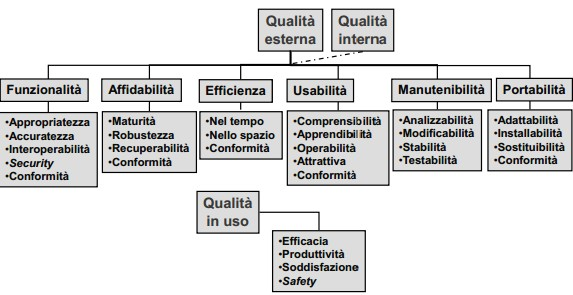
\includegraphics[scale=0.6]{imgs/isoiec_9126_2001.jpg}
  \caption{Caratteristiche di qualità software secondo il modello
    ISO/IEC9126:2001}
\end{figure}

\subsubsection{Valutazione della qualità: metriche}

Con valutazione della qualità intendiamo il processo attraverso cui, con l'uso
di metriche definite, vengono assegnati valori ad attributi di una entità su una
scala predefinita. Uno standard di valutazione della qualità è l'ISO/IEC 14598,
ora inglobato, insieme al 9126, da ISO/IEC 25000:2005.

Definiamo \strong{metrica} qualsiasi tipo di misurazione riguardante un sistema,
un processo o un documento software. Le metriche costituiscono uno strumento di
quantificazione del prodotto e del processo, e sono utilizzate per controllare i
processi software, per effettuare previsioni sugli attributi del prodotto e per
identificare componenti anomali.

\paragraph{Attributi interni e esterni}

Le metriche misurano attributi interni del sistema, ma spesso siamo più
interessati a quelli esterni. Gli attributi di qualità esterni, come
mantenibilità o usabilità, sono tipicamente difficili da misurare, poichè
dipendono da fattori soggettivi relativi all'esperienza dell'utente. Per farlo,
occorre misurare gli attributi interni e assumere che esista una relazione con
gli attributi esterni che si vogliono valutare.

Perchè la misurazione di un attributo interno del software sia utile alla
valutazione di una caratteristica esterna, occorre che

\begin{enumerate}
  \item L'attributo interno sia misurato correttamente;
  \item Il valore dell'attributo di qualità sia, in qualche modo, correlato con
    il valore che si sa misurare;
  \item La relazione sia esprimibile e validabile formalmente in termini di
    formula o modello;
\end{enumerate}

\begin{figure}[h]
  \centering
  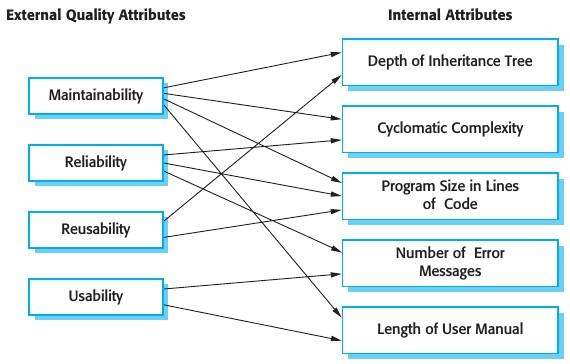
\includegraphics[scale=0.6]{imgs/int_ext_attrib.jpg}
  \caption{Relazione tra caratteristiche esterne e attributi interni del
    software}
\end{figure}

\subsubsection{Standard di qualità}

Gli standard giocano un ruolo molto importante nella gestione della qualità del
software. Essi:

\begin{itemize}
  \item Catturano e rappresentano le conoscenze, l'esperienza e le
    \frgnword{best-practice} dell'azienda;
  \item Forniscono un \frgnword{framework} per l'attuazione di \frgnword{quality
      assurance};
  \item Supportano la continuità nel momento in cui il lavoro svolto da una
    persona viene continuato da un'altra: processi standardizzati sono
    facilmente comprensibili da nuovi assunti;
\end{itemize}

Un uso errato degli standard può avere effetti negativi. E' importante che le
norme siano snelle, chiaramente complensibili e supportabili da strumenti
automatizzati.

\begin{itemize}
  \item Se gli standard sono poco comprensibili, il personale può percepirli
    come irrilevanti o bloccanti;
  \item La loro attuazione cieca può comportare eccessi di burocrazia;
  \item Senza il supporto di strumenti informatici, possono richiedere tediose
    attività manuali;
\end{itemize}


\section{Ingegneria dei requisiti} I requisiti di un sistema sono descrizioni
delle funzionalità di un sistema, i servizi che fornisce e i vincoli sulle sue
operazioni. In particolare, secondo il glossario IEEE, un requisito è:

\begin{enumerate}
  \item Una condizione (\frgnword{capability}) necessaria a un utente per
        risolvere un problema o raggiungere un obbiettivo (visione dal lato del
        bisogno);
  \item Una condizione (\frgnword{capability}) che deve essere soddisfatta o
        posseduta da un sistema per adempiere a un obbligo (contratto, standard,
        specifica, documento formale) (visione dal lato della soluzione);
  \item Una descrizione documentata di una condizione (\frgnword{capability})
        come in 1. e 2.
\end{enumerate}

\todo{slide 3/42 si riferisce alla verifica e alla validazione. inserirla nelle
sezioni relative?}

\todo{slide 4..6/42 ??}

L'attività durante il quale si delineano, analizzano, documentano e verificano i
servizi, le funzionalità e i vincoli di un sistema è chiamato \strong{ingegneria
dei requisiti}. L'ingegneria dei requisiti è parte integrante dell'ingegneria di
sistema e attività chiave del processo di sviluppo, e richiede competenze
specializzate. Rappresenta l'insieme di attività necessarie al trattamento
sistematico dei requisiti.

\paragraph{Attività}
\begin{itemize}
  \item Analisi
    \begin{itemize}
      \item Analisi dei bisogni (identificare cosa so o leggo che devo fare) e
            delle fonti (luoghi dal quale scaturiscono altri bisogni)
      \item Classificazione dei requisiti: non si vuole avere un insieme
            disorganizzato di requisiti, ma organizzarli in modo strutturato e
            ordinato.
      \item Modellazione concettuale del sistema: diagramma Casi d'Uso, che
            rappresenta il punto di vista dell'attore (qualsiasi entità esterna
            al sistema che interagisce con esso). Definisce i bisogni esterni
            del sistema.
      \item Assegnazione dei requisiti a parti distinte del sistema
      \item Negoziazione con il committente e con i sotto-fornitori: i requisiti
            devono essere concordati e negoziati con gli \frgnword{stakeholder},
            in modo che vengano fissati quelli irrinunciabili e individuati
            quelli secondari che, in mancanza di risorse, potranno essere
            scartati. Il confronto con le fonti (committente, utenti, ecc.) è
            fondamentale.
    \end{itemize}
  Durante l'attività di analisi dei requisiti è necessario equipaggiarsi, per
  metodo e per strumenti, per fare verifica e validazione.
  \item Specifica di verifica e validazione
    \begin{itemize}
      \item Predisposizione di revisione interna/esterna
      \item Predisposizione di prove e dimostrazioni
    \end{itemize}
  \item Analisi dei bisogni e delle fonti
    \begin{itemize}
      \item Propedeutica a identificazione, analisi, specifica e classificazione
            dei requisiti
    \end{itemize}
  \item Modellazione concettuale del sistema
    \begin{itemize}
      \item Partizionamento in componenti a scopo di allocazione dei requisiti
            (come nel diagramma dei casi d'uso)
      \item Non è progettazione della soluzione
    \end{itemize}
  \item Attribuzione dei requisiti a `parti'
\end{itemize}

L'analisi dei requisiti è conclusa dalla definizione di una \strong{\frgnword{
requirements baseline}}. Una baseline è un aggregato di \frgnword{configuration
item} associato a un punto di sviluppo strategico, chiamato
\frgnword{milestone}. Si raggiunge una \frgnword{requirements baseline} quando
vengono definiti tutti i requisiti che importano. La definizione della
\frgnword{requisiti baseline} costituisce il punto di fine dell'analisi dei
requisiti e di inizio della fase di progettazione.

\paragraph{Processi coinvolti}
\begin{itemize}
  \item Documentazione: serve uno strumento che renda i requisiti oggettivi,
        discutibili (oggetto plausibile di discussione) e non ambigui (uso di
        diagrammi, evitando il linguaggio naturale). La poca narrazione
        associata ai diagrammi deve essere di supporto, tecnica e sintetica, e
        appoggiarsi a un glossario per eliminare l'ambiguità dei termini.
    \begin{itemize}
      \item Studio di fattibilità
      \item Analisi dei requisiti
    \end{itemize}
  \item Gestione e manutenzione dei prodotti: i requisiti cambiano nel tempo per
        aggiunta, rimozione e estensione. Serve un insieme di regole, procedure
        e strumenti per gestire questi cambiamenti.
    \begin{itemize}
      \item Tracciamento dei requisiti: permette di sapere, per ogni passo di
            avanzamento nel progetto, a quale requisito risponde. Rappresentando
            il piano di attività come un grafo direzionato e aciclico, il
            tracciamento comunica il motivo di ciascun arco.
      \item Impostazione e gestione della configurazione
      \item Gestione dei cambiamenti
    \end{itemize}
\end{itemize}

\subsection{Studio di fattibilità}
Lo studio di fattibilità precede l'analisi dei requisiti, e si occupa di
valutare la fattibilità del progetto in termini di rischi, costi e benefici, e
decidere se sia conveniente procedere con il lavoro.
\begin{itemize}
  \item Fattibilità tecnico-organizzative: valutare se si hanno le competenze e
        gli strumenti necessari, le soluzioni algoritmiche e architetturali e le
        piattaforme idonee per l'esecuzione;
  \item Rapporto costi/benefici: valutare il rapporto tra il costo di produzione
        e la redditività dell'investimento, nei confronti del mercato attuale e
        futuro;
  \item Individuazione dei rischi: capire le complessità e le incertezze;
  \item Valutazione delle scadenze temporali;
  \item Valutazione delle alternative
    \begin{itemize}
      \item Scelte architetturali: sistema centralizzato o distribuito, modello
            client-server, ecc.
      \item Strategie realizzative: riuso o sviluppo ex-novo
      \item Strategie operative
    \end{itemize}
\end{itemize}

Lo studio di fattibilità è un'attività preliminare che non può impiegare troppo
tempo; è quindi un processo rapido, i cui risultati però non vengono scartati,
ma costituiscono una base di partenza per l'analisi dei requisiti.

\subsection{Tecniche di analisi}
\begin{itemize}
  \item Analisi dei bisogni e delle fonti
    \begin{itemize}
      \item Studio del dominio, con osservazione dei comportamenti dell'utente
            finale e dell'ambiente d'uso;
      \item Interazione con il cliente: instaurare un rapporto con il cliente
            non invadente, intelligente e strutturato, definito intervista. Le
            interviste costituiscono un dialogo da cui esce un resoconto
            approvato da entrambe le parti;
      \item Discussioni creative (brainstorming), coinvolgono tre figure
        \begin{itemize}
          \item Un gruppo di persone che discuta il problema
          \item Un `facilitatore', che aiuti la discussione a convergere in un
                tempo finito, che fissi un tempo e aiuti a valutare il risultato
                della discussione. Il facilitatore non può essere
                \frgnword{biased} e non è coinvolto direttamente nella
                discussione
          \item Una persona che tenga le minute della discussione, che ne
                registri i punti salienti
        \end{itemize}
      \item Prototipazione: può essere interna, a vantaggio del fornitore, o
            esterna, per arricchire il rapporto con il cliente; può essere
            usa-e-getta o incrementale;
    \end{itemize}
  \item Dominio, campo di applicazione del prodotto: a quali bisogni risponde, e
        quali problematiche coinvolge;
  \item Acquisizione delle competenze
    \begin{itemize}
      \item Documentazione preesistente
      \item Interviste agli utenti potenziali
      \item Studio delle soluzioni esistenti
    \end{itemize}
  \item Glossario
    \begin{itemize}
      \item Raccoglie e definisce i termini chiave del dominio
      \item Da sottoporre alla verifica e approvazione del committente
      \item Consolidato mediante uso nelle interviste
    \end{itemize}
\end{itemize}

\subsection{Classificazione dei requisiti}
E' fondamentale organizzare i requisiti in maniera strutturata e organizzata.
Suddividere i requisiti in diversi livelli di dettaglio è utile per comunicare
informazioni sul sistema a differenti tipologie di lettori.

Si può individuare una distinzione tra \strong{requisiti utente} e
\strong{requisiti di sistema}:
\begin{itemize}
  \item Requisiti utente: affermazioni, in forma di linguaggio naturale e
        diagrammi, di quali servizi il sistema dovrebbe offrire all'utente, e i
        vincoli secondo il quale dovrebbe operare;
\item Requisiti di sistema: descrizioni dettagliate delle funzioni, servizi e
      vincoli operativi del sistema. Costituiscono una documentazione esatta di
      cosa deve essere implementato.
\end{itemize}

I requisiti descrivono \strong{attributi di prodotto} o \strong{attributi di
processo}. Gli attributi di prodotto definiscono le caratteristiche del sistema;
rispondono alla domanda `cosa devo fare?'. Gli attributi di processo pongono
vincoli sui processi impiegati nel progetto (linguaggio di programmazione da
usare, strumento, metodo, ecc.); rispondono alla domanda `come devo farlo?'.

Gli attributi di prodotto esprimono
\begin{itemize}
  \item requisiti funzionali, che determinano le capacità di calcolo richieste
  al sistema (\frgnword{capabilities});
  \item requisiti prestazionali;
  \item requisiti qualitativi;
\end{itemize}

% TODO espandere.
Gli attributi di processo esprimono ulteriori requisiti extra-funzionali, che
riducono i gradi di libertà disponibili nella definizione della soluzione.

I requisiti devono essere verificabili: chi impone un requisito deve avere idea
di come accertarne il soddisfacimento; chi è chiamato a soddisfare un requisito
deve saperne valutare costo e complessità di verifica.

\begin{figure}[h!]
  \centering
  \begin{tabular}{|l|l|}
    \hline
    \strong{Tipologia di requisito} & \strong{Modalità di verifica} \\
    \hline
    Requisiti funzionali & test, dimostrazione formale, revisione \\
    \hline
    Requisiti prestazionali & misurazione \\
    \hline
    Requisiti qualitativi & verifica \emph{ad hoc} \\
    \hline
    Requisiti dichiarativi & revisione \\
    \hline
  \end{tabular}
\end{figure}

I requisiti hanno diversa utilità strategica:
\begin{itemize}
  \item Obbligatori: irrinunciabili per un qualsiasi \emph{stakeholder};
  \item Desiderabili: non strettamente necessari ma a valore aggiunto
        riconoscibile;
  \item Opzionali: relativamente utili oppure contrattabili in seguito;
\end{itemize}

I requisiti non devono essere in conflitto tra loro.

\section{Design pattern}

\subsection{Pattern creazionali}

\subsubsection{ Abstract Factory }

Il pattern \strong{ Abstract Factory } fornisce un'interfaccia per la creazione
di famiglie di oggetti correlati e dipendenti tra loro senza specificare le loro
classi concrete.

Il pattern può essere applicato quando

\begin{itemize}
  \item un sistema deve essere indipendente da come i suoi prodotti vengono
  creati, aggregati e rappresentati.
  \item un sistema deve interfacciarsi con molteplici famiglie di prodotti, dotate di
  interfaccia comune
  \item degli oggetti sono progettati per essere utilizzati insieme, e si vuole
  imporre tale vincolo
  \item si vuole esporre solo l'interfaccia di un gruppo di oggetti in una libreria di
  classi
\end{itemize}

\begin{figure}[h!]
  \centering
  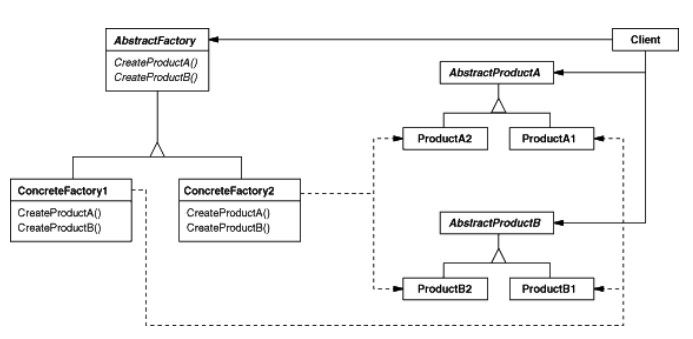
\includegraphics[scale=0.55]{imgs/abstract_factory.jpg}
  \caption{Diagramma delle classi del pattern Abstract Factory}
\end{figure}

Ogni famiglia di prodotti è creata da un'apposita ConcreteFactory, che il codice
client accede attraverso l'interfaccia di AbstractFactory. Solitamente, un solo
ConcreteFactory viene creato a run-time.

\paragraph{ Vantaggi }

\begin{itemize}
  \item Classi concrete vengono isolate dal client
  \item È possibile cambiare la configurazione di prodotti semplicemente
    cambiando la ConcreteFactory che viene istanziata.
  \item Promuove consistenza tra i prodotti, imponendo che oggetti della stessa
    famiglia vengano usati insieme.
\end{itemize}

\paragraph{ Svantaggi }

Tipicamente, l'interfaccia di AbstractFactory espone una serie di metodi
\emph{factory} che si occupano di costruire ogni oggetto della famiglia. Ogni
classe concreta specifica i suoi prodotti definendo l'implementazione di tali
metodi. Questa implementazione è semplice, ma ha lo svantaggio di richiedere un
una nuova ConcreteFactory e una completa ridefinizione dei metodi factory per
ogni famiglia di prodotti, anche se alcune famiglie differiscono tra loro solo
in alcuni dettagli.

Un altro svantaggio dell'Abstract Factory sta nella difficoltà di aggiungere
nuove classi di prodotti. L'interfaccia di AbstractFactory fissa l'insieme di
prodotti che possono essere creati, e aggiungerne di nuovi implica la modifica
della classe AbstractFactory e di tutte le ConcreteFactory che la ereditano.


\subsection{Pattern strutturali}


\printglossaries

\end{document}
